% ****** Start of file apssamp.tex ******
%
%   This file is part of the APS files in the REVTeX 4.2 distribution.
%   Version 4.2a of REVTeX, December 2014
%
%   Copyright (c) 2014 The American Physical Society.
%
%   See the REVTeX 4 README file for restrictions and more information.
%
% TeX'ing this file requires that you have AMS-LaTeX 2.0 installed
% as well as the rest of the prerequisites for REVTeX 4.2
%
% See the REVTeX 4 README file
% It also requires running BibTeX. The commands are as follows:
%
%  1)  latex apssamp.tex
%  2)  bibtex apssamp
%  3)  latex apssamp.tex
%  4)  latex apssamp.tex
%
\documentclass[%
 reprint,
%superscriptaddress,
%groupedaddress,
%unsortedaddress,
%runinaddress,
%frontmatterverbose, 
%preprint,
%preprintnumbers,
%nofootinbib,
%nobibnotes,
%bibnotes,
 amsmath,amssymb,
 aps,
%pra,
%prb,
%rmp,
%prstab,
%prstper,
%floatfix,
]{revtex4-2}
\usepackage{kotex}
\usepackage{graphicx}% Include figure files
\usepackage{dcolumn}% Align table columns on decimal point
\usepackage{bm}% bold math
%\usepackage{hyperref}% add hypertext capabilities
%\usepackage[mathlines]{lineno}% Enable numbering of text and display math
%\linenumbers\relax % Commence numbering lines

%\usepackage[showframe,%Uncomment any one of the following lines to test 
%%scale=0.7, marginratio={1:1, 2:3}, ignoreall,% default settings
%%text={7in,10in},centering,
%%margin=1.5in,
%%total={6.5in,8.75in}, top=1.2in, left=0.9in, includefoot,
%%height=10in,a5paper,hmargin={3cm,0.8in},
%]{geometry}

\begin{document}


\title{천연 색소의 추출과 무기 안료의 합성 예비보고서}

\author{서울대학교 전기정보공학부 2018-12432 박정현}
 \email{alexist@snu.ac.kr}
\date{\today}% It is always \today, today,
             %  but any date may be explicitly specified

\begin{abstract}
본 실험에서는 유기안료와 무기안료를 이용해 면섬유를 염색하고 각 안료에 의해 색깔이 나타나는 이유를 이론적으로 이해한다. 또한 유기안료를 이용해 염색한 후 매염을 하여 염료의 화학반응에 따라 색깔이 어떻게 변하는지 확이하고 이를 통해 매염제를 통해 안정도가 어떻게 변화하는지 이해한다.
\end{abstract}

%\keywords{Suggested keywords}%Use showkeys class option if keyword
                              %display desired
\maketitle

%\tableofcontents

\section{\label{sec:level1}Introudction}
\subsection{\label{sec:level2}염색}
케르세틴은 양파를 노랗게 만드는 물질이다.[1] 케르세틴의 분자식은 Fig.\ref{fig:Que}와 같다.[4] 아래의 구조에서 $\sigma$, $\pi$ 결합이 번갈아 가며 존재하여 공명하게 되고 해당 공명과 일치하는 파장의 빛이 흡수, 방출된다. 이러한 빛이 가시광선에 해당하면 우리의 눈에서는 색깔이 있는것으로 인식한다. [3]
\begin{figure}[htbp]
	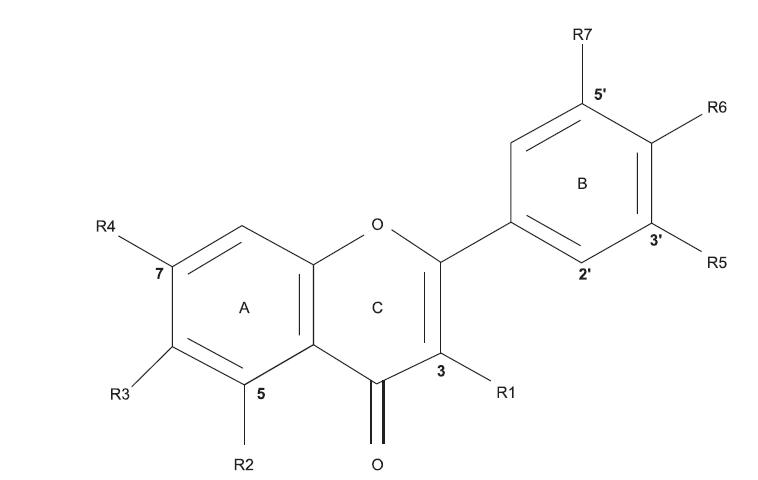
\includegraphics[width = 0.6\linewidth]{Que.png}% Here is how to import EPS art
	\caption{\label{fig:Que}케르세틴 분자 구조}
\end{figure}

반면에 무기 염료의 경우 전이금속과 양이온이 배위결합을 하면서 착화합물을 형성한다. 전이 금속은 Fig.\ref{fig:d_orbital} 같이 d-orbital에 전자들이 존재한다. 이때 양이온이 전이금속에 가까워짐에 따라 Fig.\ref{fig:energy_splitting}와 같이 전이금속 내부의 d-orbital energy가 split이 일어나게 되며 이러한 split은 central field theory를 이용해 계산할 수 있다. Split된 d level에서 전자들이 전이하면서 빛이 흡수, 방출되고 마찬가지로 이러한 빛이 가시광선의 파장대역에 해당하면 눈에서는 색깔이 있는 것으로 인식한다.[2]
\begin{figure}[htbp]
	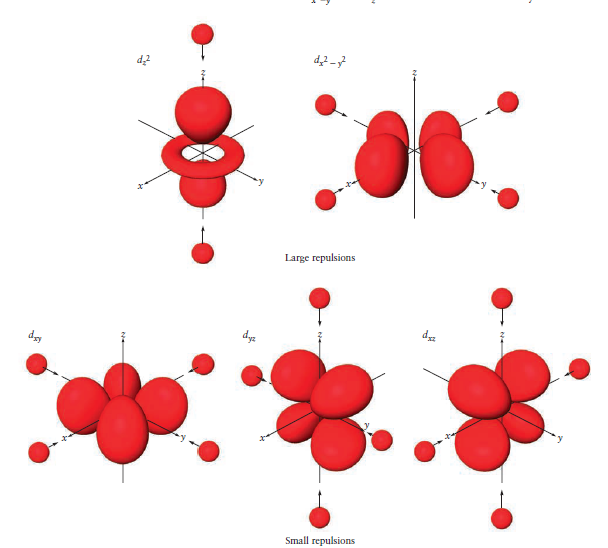
\includegraphics[width = 0.6\linewidth]{d_orbital.png}% Here is how to import EPS art
	\caption{\label{fig:d_orbital}전이금속의 d-orbital}
\end{figure}
\begin{figure}[htbp]
	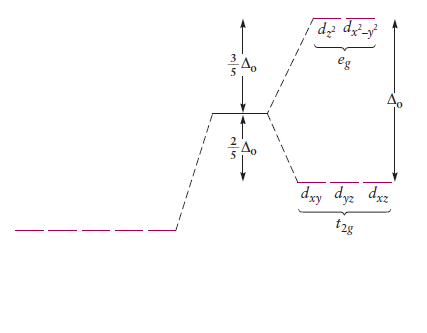
\includegraphics[width = 0.6\linewidth]{energy_splitting.png}% Here is how to import EPS art
	\caption{\label{fig:energy_splitting}배위결합에 의한 d-orbital energy split}
\end{figure}

면섬유가 polyamide 중합체인 경우 $NH$기의 양극이 케르세틴 양극과 결합할 것이다. 반면에 셀룰로우스와 같은 경우에는 $OH$기의 음극이 케르세틴의 음극과 수소결합을 하게 될 것이다.[3] 각각에 대한 그림은 Figs.\ref{fig:NH3_bond}, \ref{fig:OH_bond}와 같다. 매염을 하는 경우 금속 원자와 유기염료 분자와 배위화합물을 형성하게 된다. 이 때 매염제의 경우 $Al_{2}(SO_{4})_{3}\cdot18H_{2}O$, $FeCL_{2}\cdot nH_{2}O$와 같은 물질을 사용하며 금속이온의 리간드에 의해 발생한다. 이러한 배위화합물은 면섬유와 케르세틴의 결합을 강하게 유지할 수 있게 만들어준다.
\begin{figure}[htbp]
	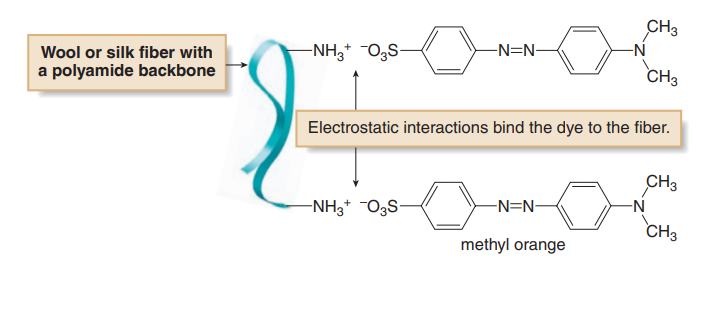
\includegraphics[width = 0.6\linewidth]{NH3_bond.png}% Here is how to import EPS art
	\caption{\label{fig:NH3_bond}염료분자와 polyamide의 결합}
\end{figure}
\begin{figure}[htbp]
	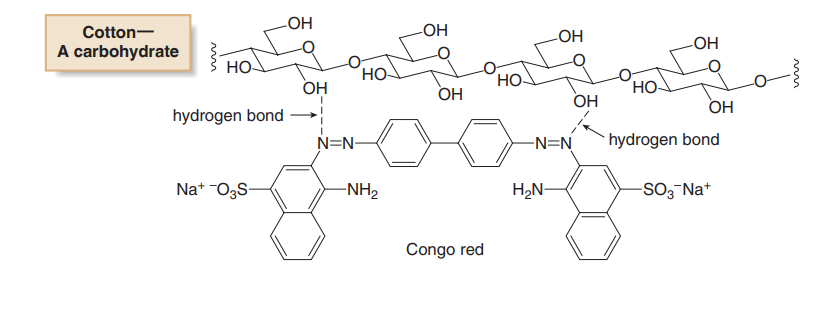
\includegraphics[width = 0.6\linewidth]{OH_bond.png}% Here is how to import EPS art
	\caption{\label{fig:OH_bond}염료분자와 carbonhydrate 분자와의 결합}
\end{figure}

\section{\label{sec:level1}Experimental}
\subsection{\label{sec:level2}천연 색소의 추출}
$100mL$ 비커, 열 교반기, 핀셋, 약수저, 종이 타월, 백반($KAI(SO_{4})_{2}\cdot 12H_{2}O$), $FeCL_{2}\cdot nH_{2}O$, $NaHCO_{3}$ 용액 ($0.2g/10mL$), 아세트산, 치자, 소목을 준비한다. 두개의 $100mL$ 비커에 $50mL$씩 물을 채운뒤 각각에 $Al_{2}(SO_{4})_{3}\cdot18H_{2}O$, $FeCL_{2}\cdot nH_{2}O$을 $1.5g$ 씩 넣는다. 이 때 각각에 표시를 한뒤 저어주면서 5분 정도 가열한다. 이후에 면섬유를 각각의 비커에 넣고 2분 가량 가열한 뒤 잘 보관한다. 이후에 $100mL$ 비커 두개에 $50mL$을 물을 가열한 뒤 한쪽에는 양파의 겉껍질을 넣고 다른 비커에는 흰껍질을 잘게 잘라 넣은 뒤 5분 가량 가열한다. 이 때 색이 색이 우려 나온 이후 건더기를 걸러 염색시 얼룩이 생기지 않도록 한다. 이후에 면섬유 두개를 흐르는 물에 적셔준뒤 두 면섬유를 각각 추출된 염액에 넣은 뒤 3분가량 가열한다. 이후에 면섬유를 종이 타월에 올려 놓은 뒤 표시한다.  사용한 염액을 $100mL$ 비커 두개에 각각 분리한다. 이후에는 $Al_{2}(SO_{4})_{3}\cdot18H_{2}O$ 용액에 담가뒀던 면섬유를 각각의 염액에 넣은 뒤 3분 가량 가열한다. 이후에 흐르는 물에 씻은 뒤 표시하고 종이타월에 올려둔다. 마찬가지로 $FeCL_{2}\cdot nH_{2}O$에 담가 가열했던 면섬유를 염액에 넣고 3분 가량 가열한다. 이후에 흐르는 물에 씻고 종이타월에 올린 뒤 표시한다.

만들어진 여 섯개의 면섬유에 아세트산을 한 두 방울 떨어뜨리고, 나머지 부분에 $NaHCO_{3}$ 수용액을 한두 방울 떨어뜨린다. 이후에 흐르는 물에 씻기고 변화를 확인한다.

\subsection{\label{sec:level2}무기 안료의 합성}
열교반기, 청량 종이, 여과지, 뷰르너 깔때기, 뷰르너 플라스크, 유리막대, 카세인, 그리고 아래 표의 물질들을 준비한다. 두 개의 시험관에 뜨거운 물을 $50mL$가량 채운 뒤 각 색깔에 해당하는 물질을 섞으면 침전이 생긴다. 뷰흐너 깔때기를 이용해 침전을 걸러서 말리고 $100mL$ 비커에 카세인을 넣은 뒤 물을 넣어 걸쭉한 반죽을 만든다. 이후에 해당 반죽을 같은 양의 색소를 넣은 뒤 넣고 잘 저어준다.
\begin{table}[]
\begin{tabular}{c|c|c} \hline \hline
반응 물질 & 침전 물질 & 침전물 색깔 \\ \hline
$0.3g K_{4}Fe(CN)_{6}$ , $0.2g CoCl_{2}$ & $CoFe(CN)_{6}$ & 회녹색 \\ \hline
$0.2g NH_{4}Fe(SO_{4})_{2}$ , $0.2g Na_{2}CO_{3}$ & $Fe(OH)_{3}$ & 갈색 \\ \hline
$0.2g NH_{4}Fe(SO_{4})_{2}$ , $0.2g K_{4}Fe(CN)_{6}$ & $KFe(CN)_{6}$ & 파란색 \\ \hline
$0.2g CoCl_{2}$ , $1.0mL Na_{2}SiO_{3}$ & $CoSiO_{3}$ & 보라색 \\ \hline
$0.2g CoCl_{2}$ , $0.2g Na_{2}CO_{3}$ & $CoCO_{3}$ & 연보라색 \\ \hline \hline
\end{tabular}
\caption{\label{tab:C18}무기 안료를 만들기 위한 물질들과 색깔들}
\end{table}

\section{\label{sec:level1}Reference}
[1] 김희준, \textit{일반화학 실험}(자유아카데미, 2016), pp.158.\\

[2] D.W. Oxtoby, H.P. Gillis, and L. Butler, \textit{Principles of Modern Chemistry} (Brooks/Cole, Australia, 2020), pp.345-348.

[3] J.G. Smith, \textit{Organic Chemistry} (McGraw-Hill Education, New York, NY, 2020), pp.988-990. 

[4] M. Materska, Polish Journal of Food and Nutrition Sciences 58, 407-413 (2008). 


\end{document}
%
% ****** End of file apssamp.tex ******
